\documentclass[11pt, letterpaper]{article}   	% use "amsart" instead of "article" for AMSLaTeX format
\usepackage{graphicx}				% Use pdf, png, jpg, or eps§ with pdflatex; use eps in DVI mode
\usepackage{amssymb}
\usepackage{amsmath}
\usepackage{url}
% Author affiliations
\usepackage{authblk}
% Allow inline lists
\usepackage[inline]{enumitem}
\usepackage[
    backend=biber,
    citestyle=authoryear,
    style=authoryear,
    autocite=inline,
    isbn=false, doi=false, url=false, eprint=false,
    uniquename=false,
    uniquelist=false,
    maxcitenames=2,
    mincitenames=1,
    maxbibnames=9
]{biblatex}

\newcommand{\beginsupplement}{%
        \setcounter{table}{0}
        \renewcommand{\thetable}{S\arabic{table}}%
        \setcounter{figure}{0}
        \renewcommand{\thefigure}{S\arabic{figure}}%
     }

% Don't print month and day in bibliography
\AtEveryBibitem{\clearfield{month}}
\AtEveryBibitem{\clearfield{day}}
% Fix biblatex behavior that writes "In: " before journal name.
\renewbibmacro{in:}{%
  \ifentrytype{article}{}{\printtext{\bibstring{in}\intitlepunct}}}


\newcommand{\eq}[1]{Eq.~(\ref{#1})}
\newcommand{\Eq}[1]{Equation~(\ref{#1})}
\newcommand{\eqs}[2]{Eq.~(\ref{#1})~and~(\ref{#2})}
\newcommand{\fig}[1]{Fig.~\ref{#1}}
\newcommand{\Fig}[1]{Figure~\ref{#1}}
\newcommand{\figs}[2]{Fig.~\ref{#1}~and~\ref{#2}}

\newcommand{\floor}[1]{\lfloor #1 \rfloor}
\newcommand{\E}[1]{\left< #1 \right>}

\DeclareMathOperator{\pmi}{PMI}
\DeclareMathOperator{\fpmi}{fPMI}
\DeclareMathOperator{\wfpmi}{wfPMI}
\DeclareMathOperator{\hilopmi}{hiloPMI}


\addbibresource{references.bib}

\title{Distinguishing multiple-merger from Kingman coalescence using two-site frequency spectra}
\author[1,2]{Daniel P. Rice}
\author[1,2,*]{John Novembre}
\author[3,4,*]{Michael M. Desai}
\affil[1]{Department of Human Genetics, University of Chicago, Chicago, IL}
\affil[2]{Department of Ecology and Evolution, University of Chicago, Chicago, IL}
\affil[3]{Department of Organismic and Evolutionary Biology, Harvard University, Cambridge, MA}
\affil[4]{Department of Physics, Harvard University, Cambridge, MA}
\affil[*]{These authors contributed equally to this work.}
\date{\today}

\begin{document}
\maketitle

\abstract{
Demographic inference methods in population genetics typically assume that the ancestry of a sample can be modeled by the Kingman coalescent.
A defining feature of this stochastic process is that it generates genealogies that are binary trees: no more than two ancestral lineages may coalesce at the same time.
However, this assumption breaks down under several scenarios.
For example, pervasive natural selection and extreme variation in offspring number can both generate genealogies with ``multiple-merger'' events in which more than two lineages coalesce instantaneously.
Therefore, detecting multiple mergers is important both for understanding which forces have shaped the diversity of a population and for avoiding fitting misspecified models to data.
Current methods to detect multiple mergers in genomic data rely on the site frequency spectrum (SFS).
However, the signatures of multiple mergers in the SFS are also consistent with a Kingman coalescent with a time-varying population size.
Here, we present a new method for detecting multiple mergers based on the pointwise mutual information of the two-site frequency spectrum for pairs of linked sites.
Unlike the SFS, the pointwise mutual information depends mostly on the topologies of genealogies rather than on their branch lengths and is therefore largely insensitive to population size change.
This statistic is global in the sense that it can detect when the genome-wide genetic diversity is inconsistent with the Kingman coalescent, rather than detecting outlier regions, as in selection scan methods.
Finally, we demonstrate a graphical model-checking procedure based on the pointwise mutual information using genomic diversity data from \textit{Drosophila melanogaster}.}

\section*{Introduction}
The genetic diversity of a population reflects its demographic and evolutionary history.
Learning about this history from contemporary genetic data is the domain of modern population genetics (see~\cite{Hahn2018a}).
The fundamental tools of the trade are simplified mathematical models, which connect unobserved quantities such as the population size to observable features of genetic data.
However, populations are complicated and, moreover, vary in their complications.
No simple model can capture the processes governing every species' evolution, and a misspecified model will generate misleading inferences.
It is therefore crucial to understand the limits of population genetics models and to assess when a model is appropriate for a particular data set.

One of the most widely used models is the Kingman coalescent~\autocite{Kingman1982, Kingman1982a, Hudson1983, Tajima1983}.
The Kingman coalescent is a stochastic process that generates gene genealogies: trees representing the patterns of shared ancestry of sampled individuals.
Inference methods use these genealogies as latent variables linking demographic parameters to genetic data~\autocite{RosenbergNordborg2002}.
The Kingman coalescent has a number of convenient properties that facilitate both analytical calculations (e.g.,~\cite{Tajima1989}) and efficient stochastic simulations (e.g.,~\cite{Hudson2002}): tree topologies are independent of waiting times; waiting times are generated by a Markov process; and neutral mutations are modeled as a Poisson process conditionally independent of the tree.
Moreover, the model can be extended to study a variety of biological phenomena including recombination, population structure, and variation in sex ratios or ploidy (see generally~\cite{Wakeley2009}).

An important application of the Kingman coalescent is inferring historical population sizes from genetic data~\autocite{SchraiberAkey2015}.
In its simplest form, the model has a single parameter, the coalescent rate, which determines the branch lengths of genealogies~\autocite{Kingman1982}.
Under many conditions, the coalescent rate is inversely proportional to the population size~\autocite{Kingman1982a}.
Accordingly, a growing or shrinking population may be modeled by a time-varying rate~\autocite{GriffithsTavare1994, GriffithsTavare1998}.
Patterns of genetic diversity depend on the ratio of the coalescent rate to other evolutionary rate parameters.
For example, the \emph{site frequency spectrum} (SFS)---the number of mutations segregating at different frequencies in a sample---is determined by the ratio of the mutation rate to the (time-varying) coalescent rate.
Kingman coalescent--based inference methods solve the inverse problem of determining the population size history that best explains particular features of the data, such as the SFS (e.g., \cite{BhaskarEtAl2015}) or variations in heterozygosity along a chromosome (e.g., \cite{LiDurbin2011}).

A serious problem for this class of inference methods is that different models of evolution generate different relationships between historical population sizes and genetic diversity.
For example, one of the basic assumptions of the Kingman coalescent is that natural selection is negligible in determining the distribution of genealogies.
When this assumption is violated, Kingman-based inference methods are misspecified.
For instance, when a beneficial mutation increases rapidly in frequency, it distorts the genealogies at nearby sites (see e.g., \cite{CoopRalph2012}).
If these ``selective sweeps'' occur regularly, they may be the dominant factor determining the distribution of genealogies.
In this case, the average coalescent rate is proportional to the number of beneficial mutations introduced per generation, which is itself \emph{directly}, rather than inversely, proportional to the population size.
It follows that the relationship between the population size and the expected number of neutral mutations in a sample is inverted: larger populations will be less diverse than smaller populations.

While the example above is extreme, it is well established that violations of the neutrality assumption can distort or mask the signatures of population size changes.
For example, \textcite{SchriderEtAl2016} recently demonstrated that several popular inference methods give misleading results in the presence of selective sweeps.
In a similar vein, \textcite{CvijovicEtAl2018}, showed that reduction of genetic diversity by purifying selection is accompanied by distortions in the SFS, leading to a false signal of population growth.
Moreover, genomic evidence from multiple species suggests that such violations of neutrality may be widespread \autocite{SellaEtAl2009, Corbett-DetigEtAl2015, KernHahn2018}.

An important extension of the Kingman coalescent is a family of models known as \textit{multiple-merger coalescents} (\cite{Pitman1999, Sagitov1999, DonnellyKurtz1999,}; reviewed in \cite{Eldon2016}), which arise in a variety of contexts both with and without selection.
Whereas in the Kingman coalescent lineages may coalesce only pairwise, multiple-merger coalescents permit more than two lineages to coalesce in a single event.
The more general class of simultaneous-multiple-merger coalescents \autocite{Schweinsberg2000, MohleSagitov2001, Sagitov2003} permits more than one distinct multiple-merger event at the same time.
multiple-merger and simultaneous-multiple-merger models are relevant for species with
``sweepstakes'' reproductive events \autocite{EldonWakeley2006, SargsyanWakeley2008},
fat-tailed offspring number distributions \autocite{Schweinsberg2003},
recurring selective sweeps at linked sites \autocite{DurrettSchweinsberg2005, CoopRalph2012},
rapid adaptation \autocite{NeherHallatschek2013, DesaiEtAl2013},
and purifying selection at sufficiently many sites \autocite{SegerEtAl2010, NicolaisenDesai2012, GoodEtAl2014}.

In each of these contexts, the coalescent timescale is not necessarily proportional to the population size.
For example, with fat-tailed offspring distributions the rate of coalescence is a power law in the population size \autocite{Schweinsberg2003}, while with linked sweeps it is determined by the rate of linked sweeps, as described above \autocite{DurrettSchweinsberg2005}.
In these settings, interpreting the level of genetic diversity in terms of an ``effective population size'' is misleading, and inferences based on the Kingman coalescent may be qualitatively incorrect.

It is therefore important to determine whether the Kingman model is appropriate for a given data set before performing demographic inference.
This task is distinct from ``selection scan'' methods designed to detect particular regions of the genome that are under selection (see~\cite{VittiEtAl2013}).
Selection scan methods typically assume that most of the genome is evolving neutrally and that the genome-wide distribution of summary statistics reflects demographic factors.
Genomic regions that are outliers from this distribution are presumed to be under selection.
In contrast, we are interested in detecting when the genome-wide background \emph{is not} well-modeled by the Kingman coalescent.

One approach to identifying multiple mergers in genomic data is to use the SFS as a summary statistic.
To this end, \textcite{BirknerEtAl2013, BlathEtAl2016} and \textcite{SpenceEtAl2016} derived methods for computing the expected SFS of (simultaneous) multiple-merger coalescents.
Further, \textcite{EldonEtAl2015} showed that it is possible to distinguish between a multiple-merger coalescent of the beta family and the Kingman coalescent with exponential growth using the SFS.
In a related approach, \textcite{RodelspergerEtAl2014} detected widespread linked selection in the nematode \textit{Pristionchus pacificus} by demonstrating that the SFS is non-monotonic, a signature of multiple mergers \autocite{NeherHallatschek2013, BirknerEtAl2013}.

However, existing methods are limited in their ability to distinguish multiple mergers from general models of population-size change.
The primary signature of multiple mergers in the SFS is an overabundance of low-frequency mutations relative to the Kingman expectation, which is also the signature of population growth.
\textcite{EldonEtAl2015} were able to reject exponential growth in favor of multiple mergers, but a more flexible model of growth may be able to fit the multiple-merger SFS (see \cite{MyersEtAl2008, BhaskarSong2014}).
The non-mononotic SFS identified by \textcite{RodelspergerEtAl2014} is a more robust signature of multiple mergers, but identifying that the SFS increases at high frequencies requires knowing the ancestral allele at each site.
High-frequency mutations are typically much rarer than low-frequency mutations, so misidentifying even a small fraction of ancestral alleles can generate a non-monotonic SFS.

Here, we propose that summary statistics based on the two-site frequency spectrum (2-SFS)---the generalization of the SFS to pairs of nearby sites \autocite{Hudson2001, FerrettiEtAl2018}---are useful for distinguishing between the Kingman coalescent with population growth and multiple-merger coalescents.
These statistics may be calculated efficiently from genomic single-nucleotide-variant data.
Furthermore, they do not require phasing, recombination maps, or ancestral allele identification and are informative even with small sample sizes.
Together, these properties make the 2-SFS useful for demographic model-checking in a wide range of species.

Following the notation of \textcite{Fu1995}, the site frequency spectrum of a sample of $n$ haploid genomes is $\left\{ \xi_i : 1 \leq i < n \right\}$, where $\xi_i$ is the fraction of sites containing a mutation with derived allele count $i$ in the sample.
In many cases, the ancestral allele is unknown and so the allele in $i$ samples and the complementary allele in $n-i$ samples are indistinguishable.
Therefore, we will mostly consider the \textit{folded} site frequency spectrum $\left\{ \eta_i = \xi_i + (1-\delta_{i,n-i}) \xi_{n-i}: 1 \leq i \leq \floor{n/2} \right\}$, where $\delta_{k,k'}$ is the Kronecker delta. %, where $\eta_i = \xi_i + \delta_{n-2i} \xi_{n-i}$.
The SFS and folded SFS can be calculated from a set of single nucleotide polymorphisms (SNPs) without knowing the physical locations of the SNPs.

In contrast, the 2-SFS is a statistic of \textit{pairs} of sites.
We define the 2-SFS,
$\left\{ \xi_{ij}(d) : d > 0; 1 \leq i, j < n\right\}$,
as the fraction of pairs of sites separated by $d$ bases for which there is a mutation with derived allele count $i$ at one site and a second mutation with derived allele count $j$ at the other site.
(Note that $\xi_{ij}(d) = \xi_{ji}(d)$ by symmetry.)
The 2-SFS has been studied for a non-recombining sites by \textcite{FerrettiEtAl2018} in a neutral model and by \textcite{Xie2011a} in a model with selection.
We define the folded 2-SFS, $\eta_{ij}(d)$, by analogy to the folded SFS,  categorizing pairs of sites by their minor allele frequencies. (For non-recombining sites, the 2-SFS is independent of the distance and so we will suppress the $d$ in our notation.)

In the limit of low per-site mutation rate ($\mu\to0$) and no recombination, all polymorphic sites are bi-allelic and the expected SFS and 2-SFS are related to moments of the genealogical branch length distribution by
\begin{align}
    \E{\xi_i} &= \mu \E{\tau_i} \label{eq:expected_sfs} \\
    \E{\xi_{ij}} &= \mu^2 \E{\tau_i \tau_j},
    \label{eq:expected_2sfs}
\end{align}
where $\tau_i$ is the total length of branches subtending $i$ leaves of a gene genealogy and $\E{\cdot}$ represents the expectation over the distribution of gene genealogies defined by a coalescent model.
Thus, the SFS and 2-SFS depend on the distribution of coalescent times as well as the distribution of tree topologies.

\textcite{Fu1995} calculated the first and second moments of the branch-length distribution for non-recombining infinite-sites locus under the standard time-homogeneous Kingman coalescent.
He found that $\E{\tau_i \tau_j} < \E{\tau_i}\E{\tau_j}$ for all $j \not\in \{i, (n-i)\}$.
This result, combined with \eqs{eq:expected_sfs}{eq:expected_2sfs}, implies a negative correlation between mutations at different frequencies: trees generating a mutation with derived allele count $i$ are less likely than average to generate a second mutation with derived allele count $j \not\in \{i, (n-i)\}$.
(There are positive correlations between mutations at complementary frequencies induced by genealogies whose root node partitions the tree into subtrees of size $i$ and $n-i$.)

\textcite{BirknerEtAl2013} extended Fu's calculation to a family of multiple-merger coalescents called beta coalescents.
This one-parameter family interpolates between the Kingman coalescent and the Bolthausen-Sznitman coalescent as the parameter, $\alpha$, ranges from 2 to 1.
Beta coalescents arise in models with fat-tailed offspring distributions \autocite{Schweinsberg2003, SteinruckenEtAl2013}, and the Bolthausen-Sznitman coalescent is the limiting distribution of genealogies in populations that are rapidly adapting or experiencing extensive purifying selection \autocite{NeherHallatschek2013}.
The calculations of \textcite{BirknerEtAl2013} show positive correlations between $\xi_i$ and $\xi_j$ for $j \not\in \{i, n-i\}$ (Figures 5 and 6 of \cite{BirknerEtAl2013}).
Thus, unlike the standard Kingman coalescent, the beta coalescent can generate positive associations between mutations with different minor allele counts.

In the following, we demonstrate that the positive associations between mutations at different frequencies distinguish the multiple-merger from the Kingman coalescent and that this distinction
\begin{enumerate*}[label=(\roman*), before=\unskip{: }, itemjoin={{; }}, itemjoin*={{, and }}]
    \item applies to Kingman coalescents with time-varying coalescent rates
    \item is robust to recombination between the sites
    \item is also a feature of forward-time models with selection
    \item can form the basis of a model-checking procedure for demographic inference methods
\end{enumerate*}.
To demonstrate these four properties, we introduce a transformation of the 2-SFS that we call frequency pointwise mutual information ($\fpmi$).
We use a combination of numerical calculations and stochastic simulations to explore the properties of this statistic under different coalescent models.
Finally, we demonstrate a graphical model-checking procedure based on $\fpmi$ using genomic diversity data from \textit{Drosophila melanogaster} \autocite{LackEtAl2015}.

\section*{Methods}

\subsection*{Frequency pointwise mutual information}

We aim to quantify the dependence between minor allele counts at a pair of sites, particularly for sites with different counts ($i\neq j$).
To do so, we define the \textit{frequency pointwise mutual information} as
\begin{align}
    \fpmi(i,j;d) = \log \frac{\E{\eta_{i,j}(d)}}{\E{\eta_i} \E{\eta_j}}.
    \label{eq:fpmi}
\end{align}
\Fig{fig:schematic} shows the steps to compute $\fpmi$ from a sample of sequences.

\begin{figure}
\centering
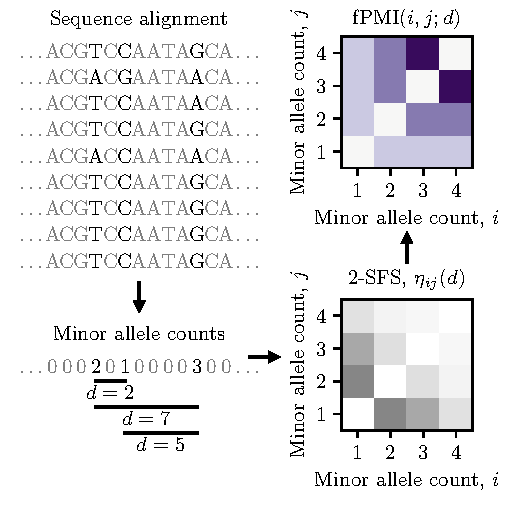
\includegraphics[scale=1]{figures/schematic.pdf}
\caption{Summarizing population genetic data with frequency pointwise mutual information ($\fpmi$). First, a sequence alignment is reduced to the minor allele frequencies and positions of segregating mutations. Then, for a given distance, $d$, the 2-SFS gives the number of pairs of sites with each combination of minor allele frequencies. Finally, $\fpmi$ is calculated from the 2-SFS according to \eq{eq:fpmi}.
 \label{fig:schematic}}
\end{figure}

In information theory, the pointwise mutual information (PMI) of a pair of random variables, $X$ and $Y$, is a transformation of the probability mass function, $p(x,y)$, given by
\begin{align}
    \pmi(x,y) = \log \frac{p(x,y)}{p(x)p(y)} = \log \frac{p(x|y)}{p(x)}
    \label{eq:pmi}
\end{align}
where $p(x) = \sum_y p(x,y)$ and similarly for $p(y)$ \autocite{ChurchHanks1990}.
PMI measures the change in the probability that $X=x$ given knowledge that $Y=y$.
When $X$ and $Y$ are independent, $\pmi(x,y) = 0$ for all $x,y$.
When $X$ and $Y$ are not independent, $\pmi(x,y) > 0$ implies that $p(x|y) > p(x)$, and $\pmi(x,y) < 0$ implies the converse.
The expectation of PMI over the joint distribution of $X$ and $Y$ is known as the mutual information of $X$ and $Y$ \autocite{CoverThomas1991}.

We can interpret the 2-SFS as a joint probability mass function over minor allele counts.
Given a coalescent model, the minor allele count at an arbitrary site is a random variable over $\{0,\ldots,\floor{n/2}\}$ with probability mass function $p(i) = \E{\eta_i}$, where we define $\eta_0$ to be the fraction of monomorphic sites.
Similarly, the minor allele counts at two sites separated by $d$ bases are random variables with joint probability mass function $p_d(i,j) = \E{\eta_{ij}(d)}$.
Comparing, \eq{eq:fpmi} with \eq{eq:pmi} shows that $\fpmi$ is the standard pointwise mutual information for pairs of minor allele counts.

This transformation of the 2-SFS has several useful properties.
First, because $\fpmi$ is based on the minor allele frequencies, we may compute it without knowing the ancestral allele.
Second, the results of \textcite{Fu1995} for the folded SFS imply that $\fpmi(i,j) < 0$ for $i\neq j$ for non-recombining sites under the time-homogeneous Kingman coalescent.
Finally, $\fpmi$ normalizes for distortions in the coalescence time distribution reflected in the single-site SFS.
In the Kingman coalescent, population-size variation alters the coalescence time distribution but preserves the distribution of tree topologies.
We will show that, because $\fpmi$ normalizes the 2-SFS by the product of single-site spectra, it is largely insensitive to the distribution of coalescence times.
Thus, $\fpmi$ primarily reflects the distribution of topologies, which distinguishes the multiple-merger coalescent from the Kingman coalescent.

Furthermore, the same normalization renders $\fpmi$ insensitive to ascertainment bias.
Variant detection methods typically compare sampled sequences to a reference sequence and ``call'' a variant site when there is sufficient evidence that at least one sample differs from the reference at that site.
As a result, the ascertainment probability, $q_i$, of a mutation is an increasing function of its true allele count $i$, skewing the expected ascertained SFS ($\E{\eta_i}_{\text{asc}} = \mu \E{\tau_i} q_i$) toward high-frequency mutations.
However, provided that variant detection at each site is approximately independent, the primary effect of ascertainment bias in \eq{eq:fpmi} is to multiply the numerator and denominator by a common factor of $q_i q_j$.
Because these factors cancel, $\fpmi$ is less sensitive than the raw SFS and 2-SFS to ascertainment effects.
% A general measure of the dependence between a pair of random variables is the \textit{mutual information} \autocite{CoverThomas1991}.
% The mutual information between random variables $X$ and $Y$ is a functional of their joint probability mass function, $p(x,y)$, defined as
% \begin{align}
%     I[p(x,y)] = \sum_{x,y} p(x,y) \log \frac{p(x,y)}{p(x)p(y)},
%     \label{eq:mutual_information}
% \end{align}
% where $p(x) = \sum_y p(x,y)$ and vice versa.
% Equivalently, the mutual information is the Kullback-Leibler divergence between the true joint distribution of $X$ and $Y$ and the joint distribution of two independent random variables with the same marginal distributions as $X$ and $Y$ \autocite{CoverThomas1991}.
% Thus, mutual information captures generic, possibly nonlinear, dependence between $X$ and $Y$.

% We would like to measure the association between alleles at particular frequencies, rather than the overall dependence between allele frequencies at nearby sites (which would be a measure of linkage disequilibrium).
% \Eq{eq:mutual_information} shows that $I[p(x,y)]$ is the expectation, relative to $p(x,y)$, of a quantity known as the \textit{pointwise mutual information}, where
% \begin{align}
%     \pmi(x,y) = \log \frac{p(x,y)}{p(x)p(y)} = \log \frac{p(x|y)}{p(x)} = \log \frac{p(y|x)}{p(y)}
% \end{align}
% \autocite{ChurchHanks1990}.
% Pointwise mutual information measures the change in the probability that $X=x$ given knowledge that $Y=y$.
% When $X$ and $Y$ are independent, $\pmi(x,y) = 0$ for all $x,y$.
% On the other hand, when $X$ and $Y$ are not independent, $\pmi(x,y) > 0$ implies that $p(x|y) > p(x)$, and conversely for $\pmi(x,y) < 0$.


\subsection*{Binned allele frequencies}

With finite data, estimates of the 2-SFS will be noisy.
This is particularly true for $i,j\gg1$ because $\E{\eta_{ij}}$ decays like $(ij)^{-1}$ for the standard Kingman coalescent \autocite{Fu1995} and faster than this in models with population size growth or multiple mergers.
We show in Results that a positive association between mutations with high minor allele counts and mutations with low minor allele counts is a signature of multiple mergers.
Thus, to detect multiple mergers, we use a binned form of the SFS and 2-SFS:
\begin{align}
    \eta_{\text{lo}}(i_c) &= \sum_{i=1}^{i_c-1} \eta_i \\
    \eta_{\text{hi}}(i_c) &= \sum_{i=i_c}^{\floor{n/2}} \eta_i \\
    \eta_{\text{hi,lo}}(d; i_c) &= \sum_{i=1}^{i_c-1} \sum_{j=i_c}^{\floor{n/2}} \eta_{ij}(d),
\end{align}
where $i_c$ is an arbitrary cutoff between high and low minor allele frequency.
Binning provides a stable estimate of the 2-SFS for large sample sizes because we may adjust $i_c$ to ensure a large number of sites in both the high--minor allele count and low--minor allele count bins.
We note that a less coarse-grained binning scheme may strike a balance between sampling noise and preserving more detailed information about allele frequencies.

We compute the pointwise mutual information of the binned distribution as
\begin{align}
    \hilopmi(d; i_c) = \log \frac
                                {\E{\eta_{\text{hi,lo}}(d; i_c)}}
                                {\E{\eta_{\text{lo}}(i_c)}  \E{\eta_{\text{hi}}(i_c)}}.
\end{align}
While we will focus on $\hilopmi$, one could similarly calculate five other pointwise mutual information statistics from the binned 2-SFS (e.g., the PMI between monomorphic sites and sites with high minor allele counts).


\subsection*{Weighted $\fpmi$}
For plotting purposes, we use a weighted version of the $\fpmi$:
\begin{align}
    \wfpmi(i,j:d) = \frac{\E{\eta_{ij}}}{\mu^2 \E{T_2}^2} \fpmi(i,j;d),
    \label{eq:wfpmi}
\end{align}
where $T_2$ is the coalescence time for a sample of size two.
The numerator of the weighting factor in \eq{eq:wfpmi} emphasizes the most common pairs of minor allele counts.
The denominator, which is proportional to the square of the expected pairwise diversity, $\Pi$, ensures that $\wfpmi$ is invariant to changes in the mutation rate and average pairwise coalescence time.

\subsection*{Computing branch-length moments}

We implemented numerical computations of the moments of the branch lengths $\E{\tau_i}$ and $\E{\tau_{ij}}$.
For the Kingman coalescent with time-varying coalescent rate, we used equations~(1)-(12) of \textcite{ZivkovicWiehe2008}.
For the beta coalescent, we implemented the recursion described by \textcite{BirknerEtAl2013}.

Functions for computing the branch-length moments are implemented in \texttt{python} and available in the \texttt{git} repository for this project (\url{https://github.com/dp-rice/multiplemergers}).
Our Kingman coalescent code can compute moments for exponentially growing and two-epoch piecewise constant models, but could be extended to allow for other models.
The formulas of \textcite{ZivkovicWiehe2008} exhibit numerical instability related to the instability described in \textcite{GriffithsTavare1994}.
Thus, these formulas are only practical for sample sizes up to $n \approx 40$.
The recursion of \textcite{BirknerEtAl2013} is $\mathcal{O}(n^4)$ and is also only practical for samples up to $n \approx 50$.

\subsection*{Coalescent simulations}

We ran coalescent simulations using a custom version of \texttt{msprime} \autocite{KelleherEtAl2016} capable of multiple mergers, based on modifications made by Joe Zhu (\url{https://github.com/shajoezhu}).
This code, together with \texttt{python} wrapper scripts and utility functions to run simulations and calculate the 2-SFS and $\fpmi$ from the \texttt{msprime} output is available at \url{https://github.com/dp-rice/multiplemergers}.

For each coalescent model, we simulated at least $10^4$ independent infinite-sites loci, each with length $d$ and per-basepair recombination rate $r$ resulting in a per-locus total recombination rate $d\,r$.
(See SI for parameter combinations.)
We chose values of $d\,r$ so that the realized values of $d\,r \E{T_2}$ varied over several orders of magnitude.
For each locus, we measured $\{\tau_i : i = 1,\ldots,n-1\}$ in the two genealogies at the ends of the locus.
We then calculated the expectations $\{\E{\tau_i}\}$ and $\{\E{\tau_{ij}}\}$ by averaging over independent loci.
These expectations allow us to calculate all of the 2-SFS statistics defined above.

\subsection*{Forward-time simulations of selective sweeps}

We simulated a model of recurring selective sweeps using the software \texttt{SLiM} \autocite{Messer2013}.
In all of these simulations, we simulated a population of 500 diploids for $10^4$ generations.
Each haploid genome consisted of a single genomic element $L=10^8$ basepairs long with recombination rate per-basepair $r = 10^{-8}$ and per-basepair mutation rate $\mu = 10^{-7}$.
We simulated two types of mutations: neutral mutations and beneficial mutations with additive effects and selection coefficient $s=0.1$.
With these parameters, $2Ns = 100$, so beneficial mutations are strongly selected and will sweep in $T_{\text{sweep}}\sim s^{-1} \log Ns \approx 50$ generations.
Such sweeps will affect a region of the chromosome $d_{\text{sweep}} \sim (r T_{\text{sweep}})^{-1} \approx 2 \times 10^6$ basepairs long.
Thus $d_{\text{sweep}} \ll L$, which will minimize edge effects of simulating a finite chromosome.

In order to vary the effects of sweeps on neutral diversity, we varied the fraction of mutations that are beneficial, $f_{\text{sel}}$, over several orders of magnitude: $f_{\text{sel}} \in \{10^{-6}, 10^{-5}, 10^{-4}, 10^{-3}\}$.
For each $f_{\text{sel}}$, we ran 100 independent replicate simulations and computed $\eta_i$ and $\eta_{ij}$ of neutral mutations averaged over all replicates.

\texttt{SLiM} parameter files, \texttt{python} wrapper scripts for parsing output, and \texttt{snakemake} files for running simulations are available at \url{https://github.com/dp-rice/multiplemergers}.

\subsection*{Analysis of \textit{D. melanogaster} data}

We analyzed sequence data from the DPGP3 data set, which consists of haploid consensus sequences from ${\sim}200$ flies, obtained via the haploid embryo method of \textcite{LangleyEtAl2011}.
The SNP calls that characterize these sequences were subjected to a variety of quality filters described in \textcite{LackEtAl2015}.
We obtained the DPGP3 consensus sequence files version 1.1 from \url{www.johnpool.net/genomes.html}.
These files contain the sequence alignments of all flies in the sample on all chromosome arms.
We also downloaded the Nov. 3, 2016 spreadsheet of inversions available at the link above.
For each chromosome arm, we excluded any samples with an inversion in that arm and then down-sampled to $n=100$ by selecting the first 100 remaining samples in alphanumeric order by sample name.
As a result, the data for each chromosome arm is from a slightly different subset of the individuals.

We calculated the average pairwise diversity, $\Pi$, as a function of position for each autosomal chromosome arm (\fig{fig:dpgp_pi}).
Pairwise diversity is high in the middle of each chromosome arm and lower near the centromeres and telomeres, in agreement with calculations by \textcite{Corbett-DetigEtAl2015}.
Our modeling---and coalescent-based demographic inference in general---assumes that the distribution of gene genealogies is homogeneous along the chromosome.
Therefore, we selected a 13-16~Mb ``central'' region of each arm with relatively homogeneous values of $\Pi$ for further analysis.
The boundary positions of these central regions are given in Table~\ref{tab:central_regions}.

In order to ensure that the segregating mutations reflect true genetic diversity and not variation in calling errors, we excluded sites with fewer than 90 of the 100 genotypes called.
This leaves over 90\% of all sites and does not substantially alter the fraction of polymorphic sites (Table~\ref{tab:called_sites}).

We fit a demographic model to the folded SFS of fourfold degenerate sites for each chromosome arm separately using \texttt{fastNeutrino} \autocite{BhaskarEtAl2015}.
Following \textcite{RagsdaleGutenkunst2017} we fit a three-epoch piecewise constant--$N$ model:
\begin{align}
    N(t) = \begin{cases}
                N_1 & 0 \leq t \leq t_1 \\
                N_2 & t_1 <  t \leq t_2 \\
                N_{\text{anc}} & t > t_2,
            \end{cases}
    \label{eq:piecewise}
\end{align}
estimating both change-points ($t_1 < t_2$) and population sizes ($N_1$, $N_2$).
We specified the ancient population size $N_{\text{anc}} = 3\times 10^5$, as in \textcite{RagsdaleGutenkunst2017}.
For all four chromosomes, \texttt{fastNeutrino} inferred similar population growth.
Fitted parameters are presented in Table~\ref{tab:DPGP_params}.
We simulated the SFS and 2-SFS under the fitted parameters using \texttt{msprime}.

In addition to the average SFS used to fit the model, we computed the average 2-SFS for pairs of sites at distances between 3~bp and 5~Kb.
Because we are using fourfold degenerate sites, we only computed the 2-SFS for distances that are multiples of three basepairs.
For comparison between data and simulations, we scale the distances in basepairs by a critical distance $d_c = (r\E{T_2})^{-1}$.
We used a genome-wide recombination rate of $r = 2 \times 10^{-8}$ per-basepair per generation \autocite{ComeronEtAl2012}.
We estimated $\E{T_2}$ by $\Pi / 2 \mu$.
For $\Pi$, we used the average pairwise diversity at fourfold degenerate sites in the central region of each chromosome arm.
For $\mu$, we used a genome-wide mutation rate of $3 \times 10^{-9}$ per-basepair per-generation \autocite{KeightleyEtAl2014}.
These estimates are not precise, but only serve to scale genetic distances to the correct order of magnitude.

A \texttt{snakemake} pipeline, \texttt{python} scripts, and \texttt{jupyter} notebooks to replicate our data processing, model fitting, simulations, and analysis of the DPGP3 data are available at \url{https://github.com/dp-rice/multiplemergers}.

\section*{Results \label{sec:results}}

\subsection*{Population growth versus the beta coalescent in non-recombining loci}

We first compared the $\fpmi$ of the Kingman coalescent with and without population growth to the $\fpmi$ of the beta coalescent, for pairs of sites without recombination.
We are interested in whether $\fpmi$ can distinguish beta from Kingman coalescent models that produce similar distortions in the SFS.
To this end, we computed a version of Tajima's D \autocite{Tajima1989} normalized to be invariant to changes in the average pairwise coalescence time: $D = (\Pi - \hat{\theta}_W) / \Pi$, where $\hat{\theta}_W$ is Watterson's theta \autocite{Watterson1975}.
Negative values of $D$ indicate an overabundance of low-frequency mutations relative to the time-homogeneous Kingman expectation.
All results are computed numerically using the results of \textcite{Fu1995}, \textcite{ZivkovicWiehe2008}, and \textcite{BirknerEtAl2013} (see Methods).

\begin{figure}
\centering
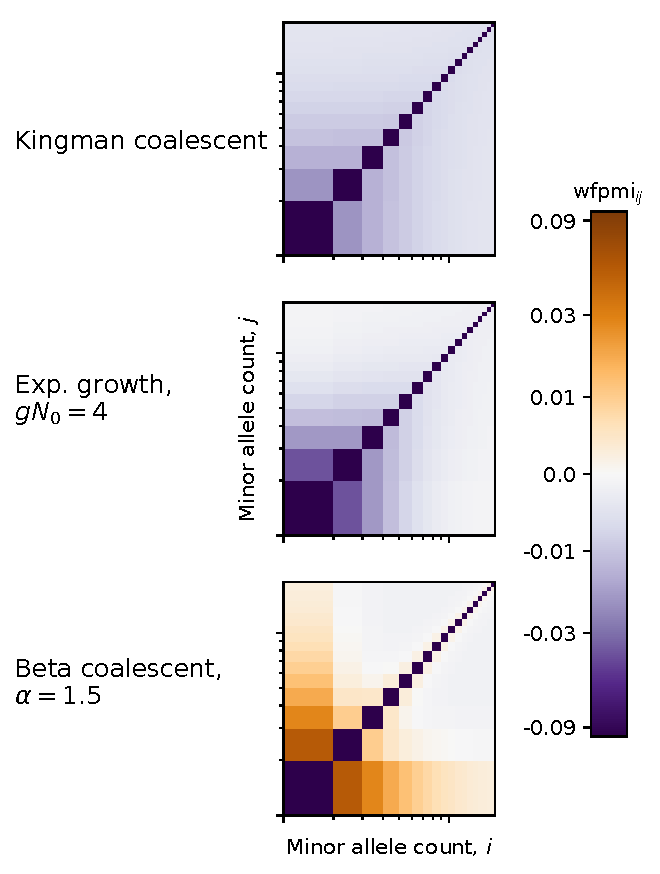
\includegraphics[scale=1]{figures/wfpmi_no_recombination.pdf}
\caption{Weighted frequency pointwise mutual information for three coalescent models: the time-homogeneous Kingman coalescent, the Kingman coalescent with exponential growth ($g=4$), and the beta coalescent ($\alpha=1.45$). For all models $n=39$. Growth and $\alpha$ parameters were chosen to generate average SFS with similar Tajima's D. The diagonal, $i=j$, is masked. \label{fig:nonrecombining_pmi}}
\end{figure}

As a first example, \fig{fig:nonrecombining_pmi} shows the $\wfpmi$ for the constant-$N$ Kingman coalescent; the Kingman coalescent with exponential growth, $N(t)=N_0 \exp(-g \frac{t}{N_0})$; and a beta coalescent intermediate between the Kingman and Bolthausen-Sznitman coalescents.
Exponential growth with $g=4$ and the beta coalescent with $\alpha=1.45$ both generate similar substantial distortions in the SFS, $D = -0.4$.
However, exponential growth does not qualitatively change the $\fpmi$.
In particular, $\fpmi_{i,j} < 0$ for all $i \neq j$, as in the constant-$N$ Kingman coalescent.
On the other hand, the beta coalescent generates positive $\fpmi$.
The effect of multiple mergers is strongest on $\fpmi$ between high and low minor allele counts.
This justifies binning the SFS and 2-SFS into high-- and low--minor allele count bins as defined above.

To generalize this finding, we computed the binned $\hilopmi$ between singletons and non-singletons ($i_c = 1$) for a range of $g$ and $\alpha$.
\Fig{fig:fpmi_vs_tajimasd} shows that as the population growth rate increases, distorting the SFS, $\hilopmi$ increases relative to the constant-$N$ Kingman, but remains negative.
On the other hand, beta coalescents that generate similar distortions in the SFS, generate larger changes in $\hilopmi$, including positive values.
Thus, the 2-SFS, and $\hilopmi$ in particular, are capable of capturing the effects of multiple mergers beyond the distortions in branch lengths.

\begin{figure}
\centering
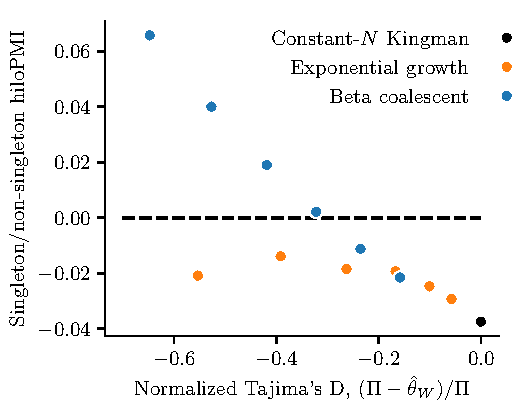
\includegraphics[scale=1]{figures/hilopmi_vs_tajimasD_no_recombination.pdf}
\caption{Pointwise mutual information between singletons and non-singletons for Kingman coalescents with exponential growth and beta coalescents. The exponential growth rate, $g$, ranges from 0.25 to 8.0 in coalescent time units. The beta coalescent parameter, $\alpha$, ranges from 1.75 (nearly Kingman) to 1.25 (nearly Bolthausen-Sznitman). \label{fig:fpmi_vs_tajimasd}}
\end{figure}

\subsection*{Pointwise mutual information between recombining sites}

We have shown in the previous section that $\fpmi$ between pairs of non-recombining sites can discriminate between the Kingman coalescent with population growth and the beta coalescent.
However, most demographic inference is performed on regions of the genome with non-zero recombination rates.
Therefore, it is important to assess the robustness of our approach to recombination between sites.

To measure the effect of recombination on $\fpmi$, we ran coalescent simulations using a version of the program \texttt{msprime} \autocite{KelleherEtAl2016} modified to allow for multiple mergers (See Methods).
In particular, we simulated a model where the marginal trees are generated by the beta coalescent process, as in our numerical calculations above.
In this model, marginal genealogies will follow the beta coalescent distribution, and the average SFS will be given by the formula in \cite{BirknerEtAl2013}.
We also simulated data from two models of population growth: exponential growth and a two-epoch piecewise-constant model.

\begin{figure}
\centering
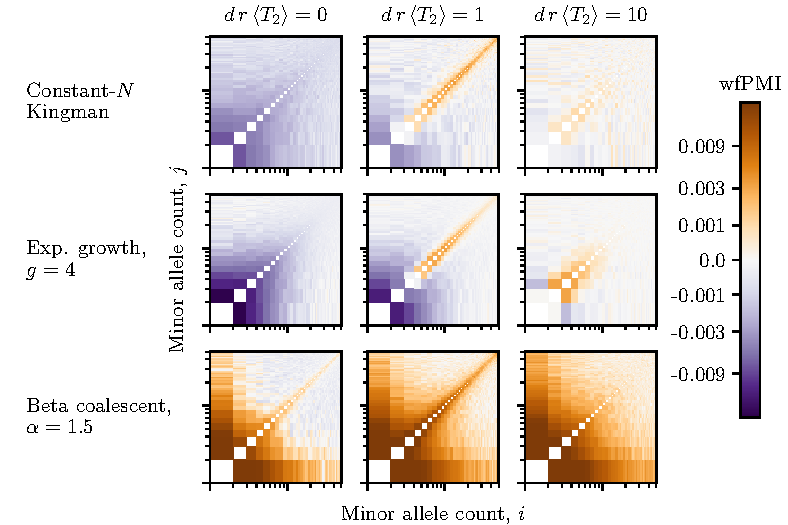
\includegraphics[scale=1]{figures/wfpmi_with_recombination.pdf}
\caption{Weighted frequency pointwise information for three recombination rates with sample size $n=100$. As in \Fig{fig:nonrecombining_pmi}, the diagonal elements are masked, and the growth and multiple-merger parameters were chosen to generate average SFS with similar Tajima's D. \label{fig:wfpmi_recombination}}
\end{figure}

\Fig{fig:wfpmi_recombination} shows the weighted $\fpmi$ for three genetic distances between sites in a constant-$N$ Kingman coalescent, a Kingman coalescent with exponential growth, and a beta coalescent.
As in the non-recombining case, the constant-$N$ and exponential-growth Kingman models have similar $\fpmi$.
In both models, $\fpmi > 0$ for $i\approx j$ for $d\,r \E{T_2} \sim 1$.
This is presumably because trees at nearby sites contain clades with similar numbers of leaves.
These positive correlations do not extend to $i \gg j$, which is the signal of multiple mergers in our binned $\hilopmi$.
On the other hand, the positive $\fpmi$ in the beta coalescent persists for $d\,r \E{T_2} > 1$.
Thus, the signal of multiple mergers in $\fpmi$ is robust to recombination.

\begin{figure}
\centering
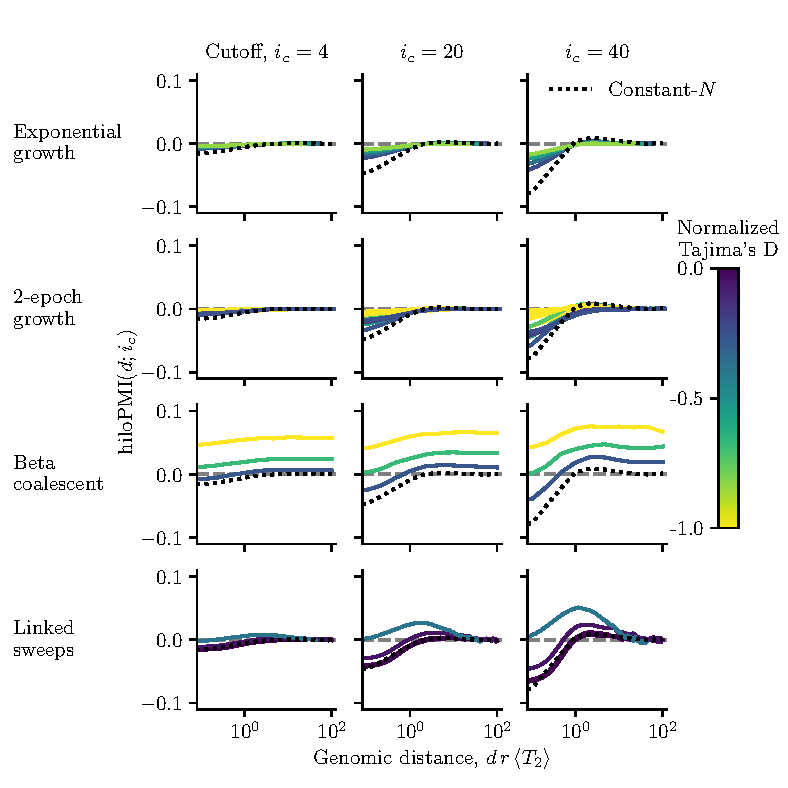
\includegraphics[scale=1]{figures/hilopmi_vs_distance.pdf}
\caption{Pointwise mutual information between high-- and low--minor allele count mutations ($\hilopmi$) versus genetic distance. Each curve represents a different combination of coalescent parameters. The first three rows show coalescent simulations in \texttt{msprime}. Exponential growth rate $g$ varies logarithmically from 1 to 8.0 in coalescent time units. Piecewise constant change-points range from 0.01 to 1 in coalescent time units, and the ratio of ancestral to modern population size ranges from 0.01 to 0.2. The fourth row shows forward-time \texttt{SLiM} simulations with selective sweeps at linked sites (beneficial mutation fraction $f_{\text{sel}} \in \{10^{-6}, 10^{-5}, 10^{-4}, 10^{-3}\}$, see Methods). Lines are colored by the distortion in the SFS, as measured by Tajima's D. The dashed line shows the constant-$N$ Kingman coalescent. \label{fig:hilo_vs_d}}
\end{figure}

\Fig{fig:hilo_vs_d} shows $\hilopmi(d,i_c)$ in both models of growth and the beta coalescent, for a range of $d\,r \E{T_2}$ and three different choices of $i_c$.
Each curve represents a particular parameter combination and coalescent model and is colored by the distortion in the average SFS (Tajima's D), which is independent of the recombination rate.
At low recombination rates, $\hilopmi$ may be greater in growing populations than in constant-$N$ populations (dotted lines), but is always less than zero, consistent with the results for non-recombining sites.
When $d\,r \E{T_2}\geq 1$, $\hilopmi$ may be slightly positive for large $i_c$, but is smaller in growing populations than in the constant-$N$ Kingman model.
In all Kingman models, $\hilopmi$ decays to zero for $d\,r \E{T_2}\gg 1$.

In contrast, the beta coalescent generates $\hilopmi$ that is consistently greater than the constant-$N$ Kingman.
As with non-recombining sites, the $\hilopmi$ is also greater in the beta coalescent model than in models of population growth that generate similar distortions in the SFS.
This is true across recombination rates and high/low cutoff minor allele counts.

These results demonstrate that $\hilopmi$ is capable of discriminating between coalescent models even when there is recombination between sites.
In particular, population growth has very little effect on $\hilopmi$, especially for $d\,r \E{T_2} \gtrsim 1$, while multiple mergers increase $\hilopmi$ across the range of $d\,r \E{T_2}$.
\Fig{fig:hilo_vs_d} also suggests that the most informative genomic distance for distinguishing multiple mergers from population growth is $d\,r \E{T_2} \sim 1$.
In a later section, we will demonstrate how to use these results to implement a model checking procedure based on plotting $\hilopmi$ as a function of genomic distance.

\Fig{fig:hilo_vs_tajD} highlights the relative invariance of $\hilopmi$ at intermediate genomic distances to population growth.
While population growth in a Kingman coalescent model can strongly distort the SFS, as measured by Tajima's D, it has very little effect on the $\hilopmi$ for sites $d\,r \E{T_2} \sim 1$ apart.
This holds for exponential as well as piecewise constant growth.
In contrast, the beta coalescent induces large positive $\hilopmi$ for the same values of Tajima's D.
The figure also shows that this result is robust to the choice of cutoff minor allele count for binning.

\begin{figure}
\centering
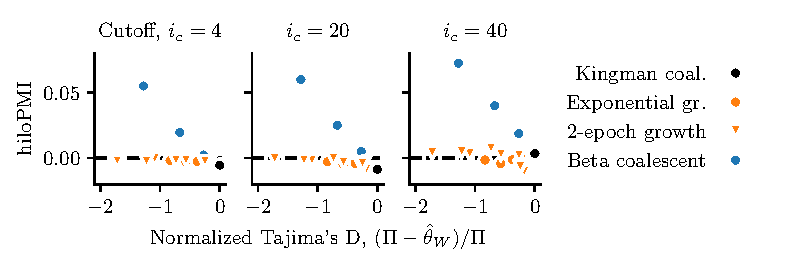
\includegraphics[scale=1]{figures/hilopmi_vs_tajimasD_recombination.pdf}
\caption{Pointwise mutual information between high-- and low--minor allele count mutations ($\hilopmi$) versus normalized Tajima's D for simulations with recombination. All values are for $d\,r \E{T_2} \sim 1$ and $n=100$. Orange points show Kingman coalescent simulations with population growth. Blue points show beta coalescent simulations. \label{fig:hilo_vs_tajD}}
\end{figure}

There is one other salient feature of \fig{fig:hilo_vs_d}: $\hilopmi$ does not decay to zero at long distances in the beta coalescent.
This behavior relates to the results of \textcite{EldonWakeley2006}, who showed that a model with ``jackpot'' reproductive events can generate infinite-range linkage disequilibrium.
Further, \textcite{EldonWakeley2006} showed that different scalings of rates of mutation, pairwise coalescence, multiple-merger coalescence, and recombination lead to different behaviors of diversity and linkage disequilibrium.
Our implementation of the beta coalescent model with recombination corresponds to a particular scaling limit where recombination does not have time to decorrelate trees during multiple-merger events, even at infinite genetic distances.
We do not expect this behavior to be universal in multiple-merger coalescents with recombination.

\subsection*{Linked selective sweeps}

Various authors have shown that natural selection can generate multiple-merger coalescents at linked neutral sites (e.g., \cite{DurrettSchweinsberg2005, CoopRalph2012, NeherHallatschek2013, DesaiEtAl2013, SegerEtAl2010}).
However, our simulations of the beta coalescent with recombination are of an explicitly neutral model.
Thus, they are at best an approximation to the selective models cited above.
It is therefore important to verify that selection at linked sites can, in fact, generate the sorts of signals in $\fpmi$ that we have detected in the beta coalescent.

To test this proposition, we performed forward-time simulations of recurring selective sweeps using the software \texttt{SLiM} \autocite{Messer2013}.
In these simulations, we simulated individual chromosomes with homogenous recombination and two types of mutations: neutral and beneficial with a fixed selection coefficient, $s$.
Both types of mutations occurred at random, uniformly distributed along the chromosome.
By varying the recombination rate, neutral and beneficial mutation rates, population size, and selection coefficient, we varied the rate of selective sweeps linked to neutral sites.

The bottom row of \fig{fig:hilo_vs_d} shows the results of these simulations.
For intermediate genetic distances, $d\,r \E{T_2} \sim 1$, the effects of linked sweeps are qualitatively similar to the effects of the beta coalescent.
That is, when sweeps are sufficiently frequent to distort the SFS, as measured by Tajima's D, they also increase $\hilopmi$.
The primary difference between the forward-time sweeps and beta coalescent simulations is that the distortions caused by sweeps decay to zero for $d\,r \E{T_2} \gg 1$.
This decay is expected because the effect of a single selective sweep on the genealogy is localized around the position of beneficial mutation.

\subsection*{Application to \textit{Drosophila melanogaster}: Coalescent model checking}

Our results above show that $\fpmi$ and its binned analog, $\hilopmi$, are useful for distinguishing population growth from the effects of multiple mergers, even when population growth generates similar distortions in the SFS.
We therefore propose the following model-checking procedure for demographic inference methods
\begin{enumerate}[label=(\roman*), before=\unskip{: }]
    \item Fit a demographic model to data.
    \item Simulate genealogies under the fitted model (using \texttt{msprime} or other coalescent simulator). Calculate the $\fpmi(d)$ and $\hilopmi(d;i_c)$ predicted by the model.
    \item Calculate $\fpmi(d)$ and $\hilopmi(d;i_c)$ from the data.
    \item Compare true to predicted statistics to evaluate model fit.
\end{enumerate}
This procedure checks whether the demographic model is consistent with a feature of the data that was not used in fitting the model.
Inconsistency suggests that the inferred $N(t)$ may be an artifact of natural selection, skewed offspring distributions, etc., rather than reflecting the true historical population size.

In this section, we illustrate the procedure outlined above by using genomic diversity data from the \textit{Drosophila melanogaster} DGPG3 panel \autocite{LackEtAl2015}.
The DPGP3 data consists of haploid consensus sequences from $\sim$ 200 wild-caught flies from a Zambian population known to be mostly free of cosmopolitan admixture.
Recently, several groups have used the DPGP3 data to estimate the population-size history of \textit{D. melanogaster} \autocite{TerhorstEtAl2017,RagsdaleGutenkunst2017}.
On the other hand, it is widely believed that the genetic diversity of \textit{Drosophila} is strongly shaped by natural selection (e.g., \cite{ElyashivEtAl2016, GarudPetrov2016}).
Thus, this data is a good candidate for demonstrating the utility of $\fpmi$ for assessing coalescent model fit.

After filtering for missing genotypes, removing chromosome arms with known inversions, downsampling to $n=100$ samples per autosomal chromosome arm, and identifying 4-fold degenerate sites, we selected the central region of each chromosome characterized by consistent high diversity (Methods).
Because the average pairwise diversity varies between arms---possibly reflecting selection or different sets of segregating inversions---we performed all subsequent calculations on each arm independently.
We fit a demographic model to the site frequency spectra of these central regions using \texttt{fastNeutrino} \autocite{BhaskarEtAl2015}.
We fit a 3-epoch piecewise-constant model, with four free parameters: two changepoints and two population size ratios.
We report our fitted parameters in Table~\ref{tab:DPGP_params}.
We then simulated under our fitted model using \texttt{msprime} and computed the expected and observed SFS, $\fpmi$, and $\hilopmi$ (\fig{fig:dpgp3}, Methods).

\begin{figure}
\centering
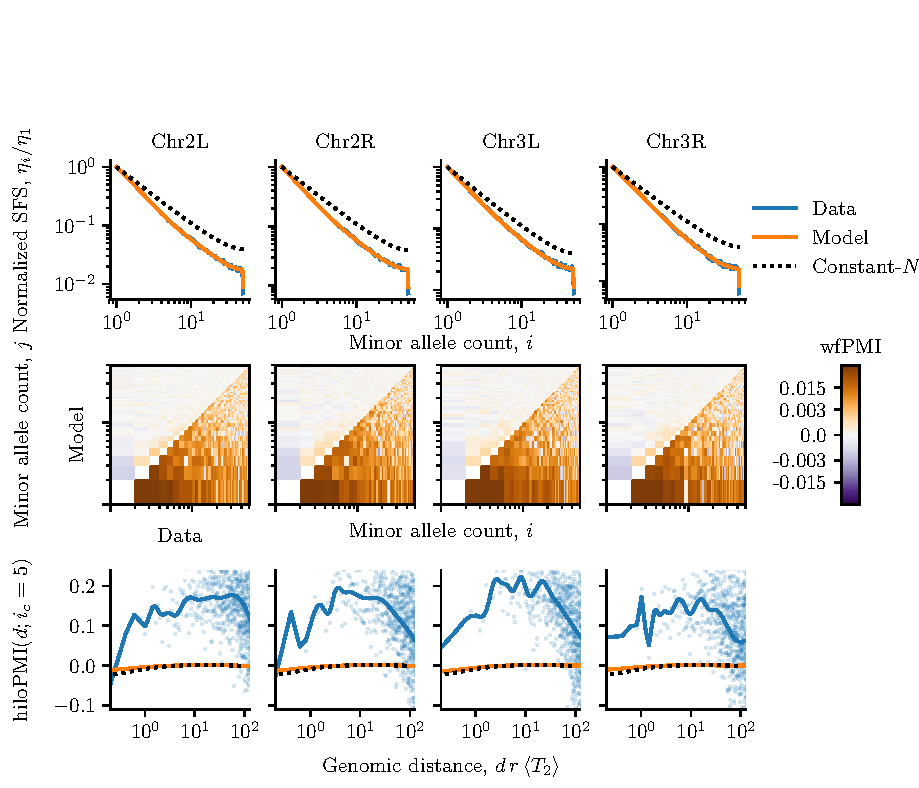
\includegraphics[scale=1]{figures/dpgp3_analysis.pdf}
\caption{DPGP3 data and coalescent model predictions. First row: observed (blue) and expected (orange) site frequency spectrum compared to constant-$N$ Kingman coalescent (dotted lines). Second row: Expected (upper triangle) and observed (lower triangle) weighted $\fpmi$ averaged over all pairs of sites less than $15 d_c$ apart. Third row: Observed (blue) and expected (orange) $\hilopmi$ versus genetic distance. Cutoff minor allele count, $i_c, = 5$. Solid blue curves show cubic spline fit. Dotted lines show the expectation under the constant-$N$ Kingman coalescent. \label{fig:dpgp3}}
\end{figure}

The first row of \fig{fig:dpgp3} shows that the expected SFS under the fit demographic models agree with the observed SFS, demonstrating that a time-varying $N(t)$ can explain this aspect of the data well.
In contrast, the second row shows the expected and observed weighted $\fpmi$ averaged over distances less than 200~bp apart, which corresponds to to $d/d_c < 15$.
Here, the data shows strong positive associations between nearby alleles at different frequencies, while the model of population growth predicts weak negative associations except adjacent to the diagonal.
This pattern extends across a range of genomic distances, $d/d_c \in (10^{-1}, 10^2)$ (\fig{fig:dpgp3}, third row).
As a result, we may conclude that the data is not well explained by the Kingman coalescent with population growth.

Note that the $\hilopmi$ decays toward zero at large distances, matching the expectation from simulations with selective sweeps rather than the beta coalescent.
However, we caution against concluding that sweeps are necessarily responsible for the deviations from the Kingman expectation.


\section*{Discussion}

We have shown that $\fpmi$ and its binned analog $\hilopmi$ are sensitive to multiple mergers, but largely invariant to population growth in the Kingman coalescent.
These properties make them well-suited for coalescent model checking.
We demonstrated a model-checking procedure on data from \textit{D. melanogaster}, which is believed to be strongly shaped by natural selection, and found evidence that population growth alone cannot explain the positive associations between high and low frequency mutations.

\begin{figure}
\centering
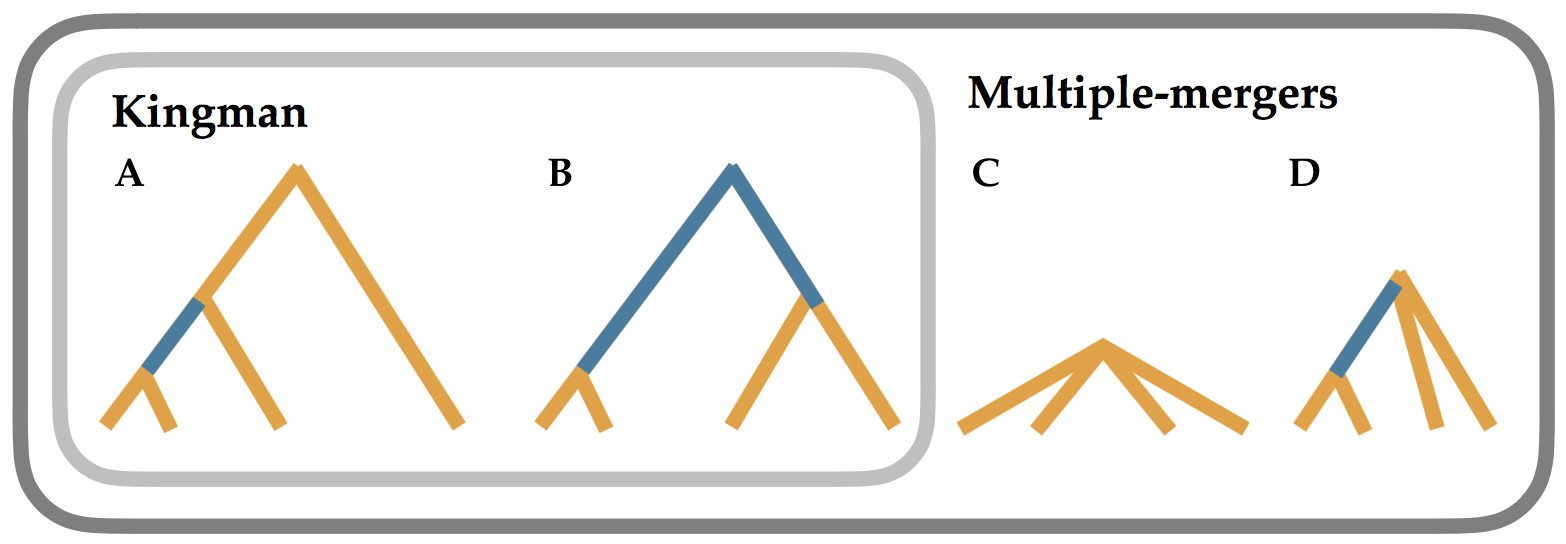
\includegraphics[width=3.5in]{figures/trees.png}
\caption{Genealogies with a sample size of $n=4$. Opportunities for singleton/tripleton mutations are in orange. Opportunities for doubletons are in blue. (Note: there is a third possible multiple-merger topology, not shown.) \label{fig:trees}}
\end{figure}

We can get an intuitive understanding for why $\fpmi$ distinguishes among coalescent models by considering a sample of four chromosomes.
In the Kingman coalescent, there are only two possible tree topologies (\Fig{fig:trees}).
Furthermore, the total branch length is independent of the topology \autocite{Wakeley2009}.
As a result, there is a trade-off between the length of branches leading to singleton/tripleton mutations on one hand, and the branch length leading to doubletons on the other.
Genealogies with topology (A) will have more opportunities for the former and loci with topology (B) will have more opportunities for the latter.
Conditional on observing a doubleton at a site, it is thus more likely that the genealogy has topology (B) and so the expected number of singletons at sites with the same genealogy is lower than average.
In terms of the 2-SFS, we have $\E{\eta_{12}} < \E{\eta_{1}} \E{\eta_{2}}$.

On the other hand, multiple mergers induce correlations between the tree topology and the total branch length.
For example, topology (C) has less opportunity for singletons \emph{and} less opportunity for doubletons than (A) or (B), even though the expected proportion of singletons is higher.
Thus, observing \emph{any mutation at all} makes topology (C) less likely and the expected number of other mutations at all frequencies higher.
If multiple-merger events are frequent enough, this effect may dominate the tradeoff between (A) and (B) so that $\E{\eta_{12}} > \E{\eta_{1}} \E{\eta_{2}}$.

\begin{figure}
\centering
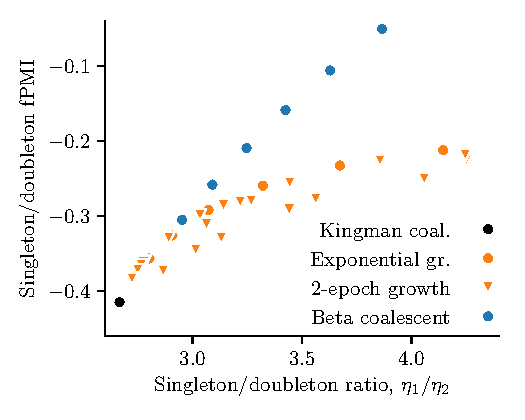
\includegraphics[scale=1]{figures/singleton-doubleton.pdf}
\caption{Distortions in $\fpmi$ vs. distortions in the SFS for $n=4$. Parameters for beta coalescents and exponential growth are as in \fig{fig:fpmi_vs_tajimasd}. For the piecewise-constant--$N$ model, the fold-change in $N$ varies from 2 to $2^4$ and the time of this change varies from $2^{-4}$ to 2 in coalescent time units. \label{fig:sdpmi_vs_sdratio}}
\end{figure}

As argued above, $\E{\eta_{12}}$ is also distorted by changes in the coalescent time distribution induced by population growth.
\Fig{fig:sdpmi_vs_sdratio} demonstrates that $\fpmi$ accounts for this fact by normalizing by the SFS.
\Fig{fig:sdpmi_vs_sdratio} plots $\fpmi(1,2)$ against the ratio of singletons to doubletons $\eta_1 / \eta_2$ for the beta coalescent and two models of population growth: exponential growth and a piecewise-constant model with two epochs.
In the latter model, we vary both the fold-change in $N$ and the time of the change.
Like Tajima's D, the singleton/doubleton ratio measures distortion in the SFS relative to the constant-$N$ Kingman coalescent.
(In fact, with $n=4$, this ratio captures \emph{all} of the distortion in the SFS.)
As with the larger sample size (\fig{fig:fpmi_vs_tajimasd}), multiple mergers generate larger distortions in $\fpmi$ than population growth does, accounting for the distortions in the SFS.
Moreover, the results for two different models of growth coincide, suggesting that the functional form of the population growth does not strongly influence $\fpmi$.

We focus here on demographic inference methods that explicitly use the Kingman coalescent model for calculations.
However, another popular class of methods are based on forward-time models, such as the Wright-Fisher model (e.g., \cite{GutenkunstEtAl2009, SheehanEtAl2013}).
We believe that $\fpmi$ is useful for model-checking with these methods as well.
This is because forward-time neutral models each have an associated dual coalescent model \autocite{Etheridge2011e}, which can be used to compute the expected $\fpmi$ as outlined in this paper.
Furthermore, non-neutral models also generate predictions about the 2-SFS and thus $\fpmi$.
In principle, any fitted model that allows calculation or simulation of the 2-SFS may be checked using $\fpmi$.
However, the suitability of $\fpmi$ for discriminating among arbitrary families of models is unknown.

In this paper, we have outlined a graphical model-checking procedure in the spirit of \textcite{Anscombe1973}.
One could extend our work to implement a formal hypothesis-testing framework for rejecting the Kingman coalescent model best-fit according to some inference method.
Numerical calculations would require higher moments of the branch-length distribution, which may be computationally intractable for large samples.
On the other hand, it would be straightforward to develop a bootstrap-style procedure, using coalescent simulations to estimate the variance in test statistics under the fit model.
In any case, we believe that it would be useful for simulation packages such as \texttt{msprime} and population genetics analysis libraries to include standard functions for computing the 2-SFS, $\fpmi$, and $\hilopmi$.
We provide such functions in the GitHub repository associated with this paper.

Our coalescent simulations implement a particular version of the multiple-merger coalescent with recombination.
However, the precise correspondence between this model and any particular forward-time process is unclear.
In order to compare with our numerical calculations based on \textcite{BirknerEtAl2013}, we use the beta coalescent for the distribution of marginal genealogies, but the explicit forward-time models that have been studied by others generate simultaneous multiple mergers.
(See e.g., the \cite{DurrettSchweinsberg2005} model of selective sweeps, but note that our forward-time simulations suggest that this distinction is not important to our main results.)
Moreover, the long-range correlations observed in \fig{fig:hilo_vs_d} likely depend on an implicit choice regarding the scaling of recombination, coalescent, and multiple-merger rates \autocite{EldonWakeley2006}.
These issues are poorly understood, and more theoretical work is required to understand the interactions between multiple mergers and recombination.

An interesteing potential future empircal application of our work would be to use $\fpmi$ to assess the evidence for variation in multiple-merger coalescence within genomes and between species.
For example, one could compute the $\fpmi$ in different regions of a large genome and look for a relationship between the strength of non-Kingman coalescence and genomic properties such as the recombination rate and functional density.
Alternatively, one could survey multiple species using a data set such as the diversity data compiled by \textcite{Corbett-DetigEtAl2015}.
Either would reveal new information about the suitability of population genetic models, and the forces that determine genetic diversity.

\subsection*{Acknowledgements}
D.P.R. was supported by the Chicago Fellows Program of the University of Chicago.
J.N. acknowledges support for this work from NIH grants GM108805 and HG007089.
M.M.D. acknowledges support from the Simons Foundation (Grant 376196), grant DEB-1655960 from the NSF, and grant GM104239 from the NIH.
This work was completed in part with resources provided by the University of Chicago Research Computing Center and Harvard Faculty of Arts and Sciences Research Computing Center.
We thank
Arjun Biddanda,
Maryn Carlson,
Ivana Cvijovi\'c,
Ben Good,
Dick Hudson,
Evan Koch,
Joe Marcus,
Richard Neher,
Matthias Steinr\"ucken,
John Wakeley,
and Aleksandra Walczak for helpful discussions and comments on the manuscript.

\subsection*{Competing interests}
The authors have no competing interests.

\printbibliography

\clearpage
\beginsupplement
\section*{Supplementary Figures and Tables}

\begin{figure}[ht!]
\centering
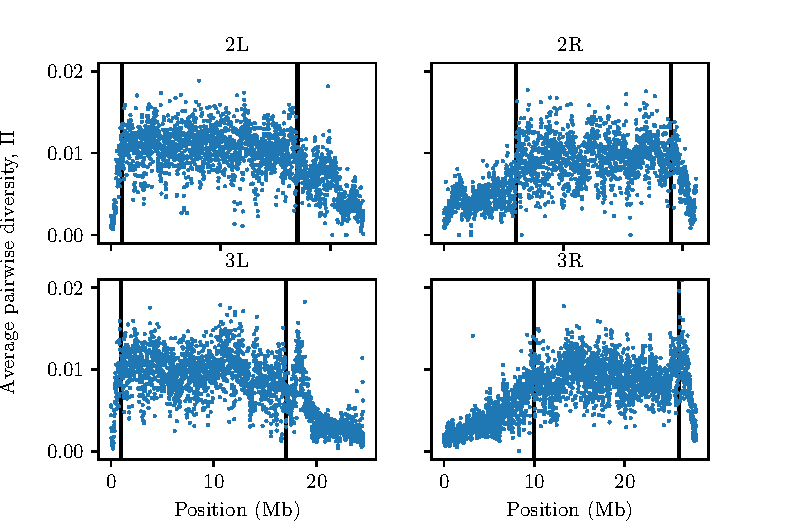
\includegraphics[scale=1]{figures/pi_vs_position.pdf}
\caption{Average pairwise diversity, $\Pi$, of 100 haploid samples from DPGP3 panel. Each point represents the average over a 10~Kb window. Vertical lines show the boundaries of the central regions defined in Table~\ref{tab:central_regions}.
\label{fig:dpgp_pi}}
\end{figure}

\begin{table}[ht!]
  \begin{center}
    \caption{Boundaries of the homogeneous central regions of chromosomes (shown in \fig{fig:dpgp_pi}).}
    \label{tab:central_regions}
    \begin{tabular}{l|r|r} % <-- Alignments: 1st column left, 2nd middle and 3rd right, with vertical lines in between
      \textbf{Chr.} & \textbf{Start position (Mb)} & \textbf{End position (Mb)}\\
      \hline
      2L & 1 & 17\\
      2R & 6 & 19\\
      3L & 1 & 17\\
      3R & 10 & 26
    \end{tabular}
  \end{center}
\end{table}

\begin{table}[h!]
  \begin{center}
    \caption{Fraction of sites with at least 90 genotyped samples}
    \label{tab:called_sites}
    \begin{tabular}{l|r|r} % <-- Alignments: 1st column left, 2nd middle and 3rd right, with vertical lines in between
      \textbf{Chr.} & \textbf{All sites} & \textbf{Polymorphic sites}\\
      \hline
      2L & 0.913 & 0.924 \\
      2R & 0.922 & 0.925 \\
      3L & 0.919 & 0.920 \\
      3R & 0.933 & 0.936
    \end{tabular}
  \end{center}
\end{table}

\begin{table}[h!]
  \begin{center}
    \caption{Piecewise-constant model parameters fit to the SFS of each chromosome arm (see \eq{eq:piecewise}, $N_{\text{anc}}=3 \times 10^5$).}
    \label{tab:DPGP_params}
    \begin{tabular}{l|r|r|r|r} % <-- Alignments: 1st column left, 2nd middle and 3rd right, with vertical lines in between
        \textbf{Chr.} & \textbf{$N_1 (\times 10^5)$} & \textbf{$N_2 (\times 10^5)$} & \textbf{$t_1 (\times 10^4)$} & \textbf{$t_2 (\times 10^4)$}\\
        \hline
        2L & 10.7 & 4.6 & 2.8 & 39.9 \\
        2R &  9.1 & 3.9 & 1.6 &  8.8 \\
        3L &  7.3 & 3.8 & 1.3 &  6.4 \\
        3R &  9.7 & 5.1 & 2.2 &  8.6
    \end{tabular}
  \end{center}
\end{table}

\end{document}
